
\chapter{基于条件随机场的显著性区域检测}
\section{引言}
\subsection{研究背景}
视觉显著性是由于物体、人或者像素相较于其近邻在某种特征上更为突出,从而吸引人眼注意力的一种特性。视觉显著性的信息可以有益于其他很多应用,比如图像检索\cite{tsai2012hierarchical}\cite{fang2012effective},图像的自动裁剪\cite{shechtman2013methods}\cite{deigmoeller2010context},自适应图像压缩\cite{christopoulos2000jpeg2000},以及图像分割\cite{jiang2011automatic}\cite{han2006unsupervised},等等。

正是由于其广泛的应用场景,显著性区域检测吸引了各个领域的众多学者。目前绝大多数算法都是自底向上的计算模型,通过计算局部或者全局对比度来生成显著图。

对于基于全局对比度的方法,一个区域的显著度是通过计算其与整个图像其他区域的差异度来得到的。在Zhai和Shah的工作中\cite{zhai2006visual},一个像素的显著性是通过计算其与整幅图像中其它像素的对比度来得到的,由于时间复杂度的问题,他们仅仅采用了亮度信息而忽略了其他颜色通道。显然,仅仅通过亮度信息来计算像素之间的差异性是一个非常粗略的抽象。Cheng等人\cite{cheng2011global}完善了这个工作,他们尝试使用完整的颜色信息去评估像素之间的差异性,为了降低计算复杂度的同时尽量减少失真,他们引入了直方图加速和彩色空间平滑两个工具。他们的方法在性能上远远超越了Zhai的方法。

基于局部对比度的方法则通过计算图像区域的独特性来得到其显著度,一般是计算区域与周围一个小的邻域的差异性。这个计算模型非常符合生物视觉特性,由Koch和Ullman等人最先提出\cite{koch1987shifts},之后由显著性区域检测领域的先驱者Itti等人加以完善\cite{itti1998model},将模型改为计算在多尺度下的中心-周围差异,并取得了良好的效果。在Ma和Zhang等人的工作中\cite{ma2003contrast},使用模糊集理论(fuzzy growing)改良了该算法,取得了更好的结果。其他很多学者,包括Harel等人\cite{harel2006graph},以及Liu等人\cite{liu2011learning},都将局部对比度作为一个很重要的特征。

\subsection{研究动机}
尽管基于局部对比度和全局对比度的方法都能取得一定的效果,但这两类方法都存在先天的缺陷。基于全局对比的方法由于是在全局域计算对比度,因此相同颜色的像素必然会被赋予相同的显著值,不管他们是处于前景还是背景中,这显然没有考虑到各个像素所处的周围环境;基于局部对比度的方法虽然考虑了像素的周边环境,但是却倾向于赋予区域边缘更高的显著度,在邻域缩小到一定程度时,其退化为边缘检测算子。在我们的工作中,我们希望有一种显著性区域检测算法能达到如下效果:
\begin{enumerate}
\item 能够均匀的高亮整个显著区域,从而有利于后续处理,完整的分离出显著区域。
\item 能根据区域在不同背景下,赋予不同的显著值,从而区分前景与背景中具有相同颜色的像素。
\item 算法尽量鲁棒,能针对各种不同场景的图像均具有一定的效果。
\end{enumerate}
在我们的研究中发现,局部和全局的显著性区域检测算法在某些方面是互补的,如果我们能够有机的结合不同的特征,应该可以得到更好,更鲁棒的结果。

\begin{figure}
\centering
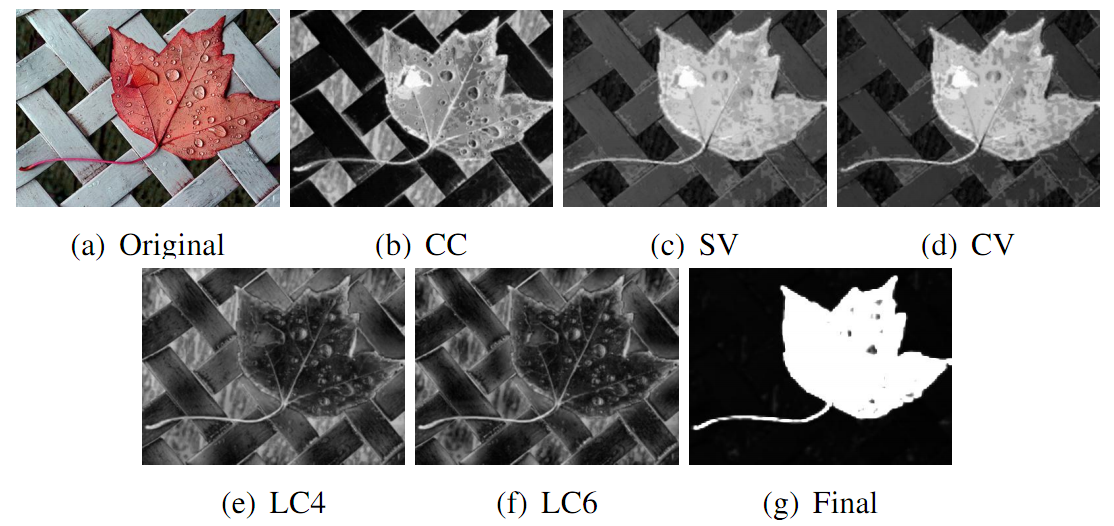
\includegraphics[width=\textwidth]{crf_example.png}
\caption{通过结合多个特征产生显著图}\label{fig:crf_example}
\end{figure}

\subsection{解决方法概要}
通过对以往经典方法的观察,我们意识到,单独依靠某一类方法,将会存在先天的不足与缺陷。在我们的方法中,首先提出了多种显著性特征产生不同的显著图(包括全局颜色对比度,全局颜色紧致度,全局颜色中心度,两种尺度下的局部颜色对比度),然后我们通过条件随机场(CRF)有机的结合这些特征,并结合相邻像素之间的关联性(相邻且相似的像素应该具有相近的显著度),达到了提高检测准确度的目的,如图\ref{fig:crf_example}所示,由原图像(a),在不同的特征下,我们产生了5副显著图,通过训练好的条件随机场模型,我们得到了最终的显著图(g),可以看出,我们的方法能够产生高质量,区域连续的显著图。

\section{显著性特征}
\subsection{全局颜色对比度}
\begin{figure}[h]
\centering
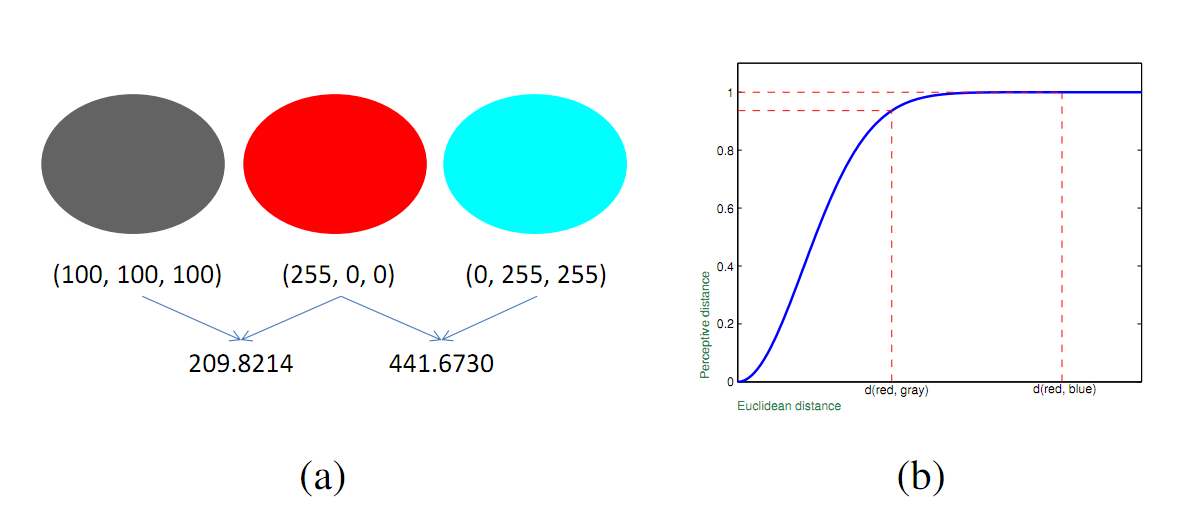
\includegraphics[width=\textwidth]{color-measure.jpg}
\caption{a.欧式距离度量颜色的不足 ~~b.使用感知距离度量颜色的效果}\label{fig:color_measure}
\end{figure}
与以往基于全局对比度的方法不一样的是,我们对颜色差异的度量进行了更加深入的研究。如图\ref{fig:color_measure}.a所示,三种颜色,从人眼看来,差别都非常大,大多数人都只能说这三种颜色差异很大,却无法区分哪两种颜色之间的差异更大。然而,如果使用欧式距离进行度量,红色与蓝色的差异是红色与灰色差异的两倍,这显然是不符合人眼对色彩的感知的,使用这种不符合人眼感知的度量方式进行对比度的计算,效果上必然也会存在一定差异。

因此,我们提出了基于人眼感知的色彩差异度量方法。如下所示,我们将两种颜色的差异度定义为:
\begin{equation}
  D(c_l, c_j) = 1 - exp(-\frac{d(c_l, c_j)^2}{2\sigma}) \label{eq:per}
\end{equation}
其中$d(c_l, c_j)$代表颜色$c_l$与$c_j$之间的欧式距离,$\sigma$表示该图像中颜色的方差。如图\ref{fig:color_measure}.b所示,使用我们提出的感知距离度量后,这种差异将更加符合人眼的认知。

在这个定义下,我们把基于全局颜色对比度的显著度定义为一个像素与图像中所有其他像素的差异:
\begin{equation}
  S_{cc}(I_k) \propto \sum_{\forall{I_i \in I}} D(I_k, I_i) ,\label{eq:u}
\end{equation}
很显然,从公式\ref{eq:u}中可以看到,相同颜色值的像素必然具有相同的显著值,因此,我们可以将公式变为如下形式,以便加速计算过程:
\begin{equation}
  S_{cc}(I_k) \propto \sum_{j=1}^{n} f_j D(c_l, c_j),
\end{equation}
其中$c_l$代表像素$I_k$的颜色向量,$n$代表不同颜色的数量,$f_j$代表颜色$c_j$在图像I中出现的频率。
使用公式\ref{eq:per}中对颜色差异的度量,我们得到最终的显著值计算公式:
\begin{equation}
  S_{cc}(I_k) \propto \sum_{j=1}^{n} f_j D(c_l, c_j),
\end{equation}
其中$D(c_l, c_j)$即代表颜色$c_l,c_j$之间的感知差异,$S_{cc}$代表像素$I_k$的显著度。

\subsection{全局颜色紧致度}
\begin{figure}
\centering
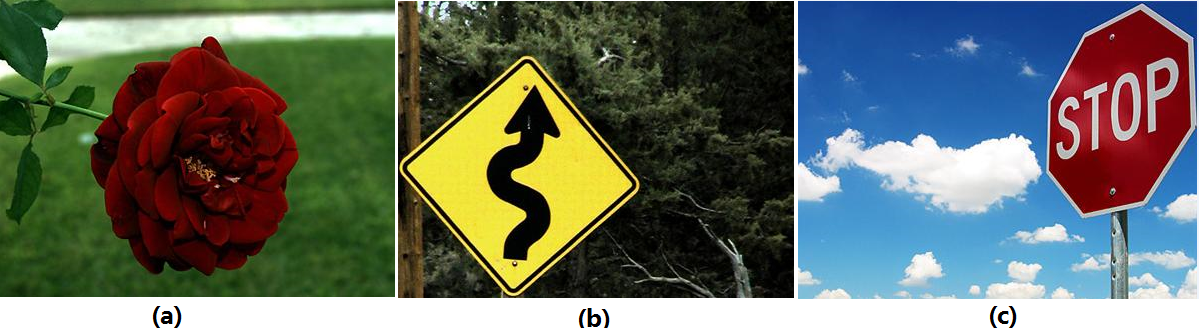
\includegraphics[width=\textwidth]{color_center.png}
\caption{颜色紧致度示例}\label{fig:color_center}
\end{figure}
除了颜色对比度,还有一些空间信息可以用来区分前景和背景像素(即显著区域与非显著区域)。根据我们的观察,显著区域的像素点通常在空间位置上分布比较紧致,而背景像素则在图像中分散开来。如图\ref{fig:color_center}(a)所示,红色花朵为显著区域,红色相对的集中于同一区域,表现为更加紧致集中,(b)(c)两图可以观察到类似的现象。概括来讲,这三图的显著区域的颜色相对分布集中,而背景像素的颜色则分布较为杂乱。在我们的全局颜色紧致度中,我们使用某种颜色的像素在空间位置上的方差来衡量像素的显著性,方差越小,说明颜色越倾向于集中分布在某一块区域,我们认为它越有可能是属于显著性区域的像素。
\begin{equation}
  U_{sv}(I_k) \propto \frac{1}{m}\sum_{i=1}^{m}(x_{c_l}^{(i)} - \bar{x}_{c_l})^2 + (y_{c_l}^{(i)} - \bar{y}_{c_l})^2 \label{eq:u0}
\end{equation}
\begin{equation}
  S_{sv}(I_k) = 1 - U_{sv}(I_k) \label{eq:u1}
\end{equation}
其中$c_l$是像素点$I_k$的颜色向量,$m$是$c_l$颜色的像素数量,$\{x_{c_l}^{(i)},y_{c_l}^{(i)}\}$是这些像素的空间位置坐标,$\{\bar{x}_{c_l},\bar{y}_{c_l}\}$则是他们的平均坐标。$U_{sv}(I_k)$代表了像素点是非显著的程度,我们把它归一化到0和1之间,然后通过式\ref{eq:u1}就可以得到图像的显著图。

\subsection{全局颜色中心度}
与全局颜色紧致度类似,我们观察到,人眼倾向于注意位于图像中心的物体和区域,也就是说,空间分布上越靠近图像中心的颜色,越有可能成为显著性区域。因此,我们使用如下式子定义:
\begin{equation}
  U_{cv}(I_k) \propto \frac{1}{m}\sum_{i=1}^{m}(x_{c_l}^{(i)} - x_c)^2 + (y_{c_l}^{(i)} - y_c)^2
\end{equation}
\begin{equation}
  S_{cv}(I_k) = 1 - U_{cv}(I_k) \label{eq:u2}
\end{equation}
其中$\{x_c, y_c\}$代表了图像中心的坐标,其他符号的含义与上节类似。同样的,我们把$U_{cv}(I_k)$归一化到0和1之间,那么,最终显著值由式\ref{eq:u2}得到。

\subsection{局部颜色对比度}
为了克服全局特征存在的一些固有问题,我们加入了局部颜色对比度作为补充。我们把局部颜色对比度定义为像素点与其周围局部区域内其他所有像素点的颜色对比度。定义如下:
\begin{equation}
  c_{i,j} = D\left [v, \frac{1}{N} \sum_{q=1}^{N}v_q \right ]
\end{equation}
其中$c_{i,j}$代表位于 $(i,j)$坐标的像素点的颜色,$N$代表了局部区域$R$中像素点的个数,$v$代表与像素点相关的颜色向量,颜色差异$D$即为我们先前定义的颜色感知距离。为了检测不同scale下的显著性区域,我们将区域$R$取两个不同大小,分别计算显著值,作为两个不同的显著图的结果。

\subsection{全局特征计算加速}
由于全局特征需要计算所有颜色在全局环境下的特征,而整个颜色空间十分巨大,对于高分辨率的图像来说,计算量更是大的不可忍受,为了加速全局特征的计算,我们采用了Cheng\cite{cheng2011global}的两个方法,即色彩向量量化与色彩空间平滑。

\textbf{色彩向量量化:} 在我们的实现中,首先将每个彩色通道量化为16个不同的值,这样就将整个颜色空间的色彩数量减少到$16^3 = 4096$。为了进一步减少颜色数量,我们选取占整个图像像素数量95\%的颜色,其他颜色则采用这些高频出现的颜色替代。最终,颜色的数量能够较少到100种左右。

\textbf{色彩空间平滑:} 在量化之后,会产生明显的人工量化痕迹,比如两个相似的颜色可能被量化为不同的颜色值,从而对最终的显著图的准确性产生一定的影响。为了尽量较少这种影响,我们采用相似颜色的加权平均显著值来平滑显著图。具体如下:
\begin{equation}
  S'(c_l) \propto \sum_{j=1}^{n} exp(-\frac{d(c_l, c_j)^2}{2\sigma})S(c_j)
\end{equation}
其中,$exp(-\frac{d(c_l, c_j)^2}{2\sigma})$是对颜色$c_l$和$c_j$的距离度量。

\section{条件随机场结合多特征方法}
现在我们可以得到5副显著图(3副全局特征,2副在不同尺度下的局部特征),既然每个显著图都是基于不同的假设与特征,那么如果能将他们结合起来就很有可能能够提高检测的准确性\cite{borji2012salient}。但是简单的对他们进行加和平均或者对应像素点相乘并不是一个好主意,因为在这种无权重的情况下,表现较好的显著图会被表现差的显著图拉低性能\cite{gopalakrishnan2009salient}。而且由于相邻像素点之间存在相互作用,单独的去评估一个像素点的显著图显然是不妥当的。在这种考虑之下,我们采用了条件随机场(CRF)这一强大的工具帮助我们结合多个显著性特征。事实上,我们描述的CRF模型与Mai等人提出的模型\cite{maisaliency}非常相似,不同的是,Mai的模型用来将其它学者提出的方法进行融合,而我们的模型用来直接将我们提出的特征进行融合。下面将对我们的模型进行描述。

\subsection{条件随机场简介}
条件随机场是一种概率图模型。不同于传统的代数解析式模型,概率图模型提供了模型的直观图形表示,并且为模型的训练求解提供了通用的方式,概率图模型具有以下优点\cite{bishop2006pattern}:
\begin{enumerate}
\item 概率图模型提供了一种简单有效的方式来可视化概率模型,同时更有利于设计新的模型。
\item 通过对图的观察,可以清楚的发现模型的一些特性,比如条件独立等等。
\item 对于复杂的模型,Inference和Learning都是非常困难的。而概率图可以将这些过程以图操作来表示,在某种程度上简化了模型的推测和学习。
\end{enumerate}

\begin{figure}
\centering
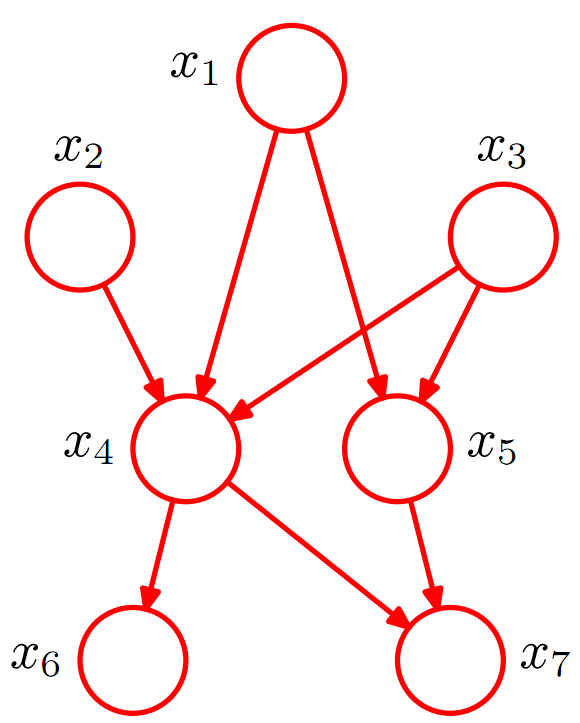
\includegraphics[width=0.5\textwidth]{graph_model.png}
\caption{图模型示例}\label{fig:graph_model}
\end{figure}

如图\ref{fig:graph_model}所示,这是一个复杂的概率模型,如果使用代数式表示,该模型的联合概率为:
\begin{equation}
P = p(x_1)p(x_2)p(x_3)p(x_4|x_1,x_2,x_3)p(x_5|x_1,x_3)p(x_6|x_4)p(x_7|x_4,x_5)
\end{equation}
显然,倘若使用传统的代数式表达如此复杂的模型,很难从代数式中观察到模型的特性,更不用说去求解、学习这样一个模型了。而如果使用图\ref{fig:graph_model}概率图来表达这个模型,则显得非常直观,节点之间的连线代表了条件独立性,而通过一些规则,我们可以轻易的写出其他条件概率表达式。

条件随机场属于无向图模型,是马尔科夫随机场在条件概率下的表达:
\begin{equation}
p(y|x,w)=\frac{1}{Z(x,w)}\prod_c \psi_c(y_c|x, w)
\end{equation}
条件随机场可以被看做是罗吉斯特回归的结构化输出的扩展\cite{murphy2012machine},我们通常使用log-linear的假设来表达potentials:
\begin{equation}
\psi_c(y_c|x,w)=exp(w_c^T \phi(x,y_c))
\end{equation}
其中$\phi(x,y_c)$是由全局输入$x$和局部标签$y_c$产生的特征向量。条件随机场(CRF)相较于马尔科夫随机场(MRF)的优势在于它是一个判别式模型,而非生成式模型,判别式模型直接对问题进行分类,准确率通常更高。

\subsection{建模目标}
为了有效利用各个显著性特征的优势,同时又保证高质量的显著图在融合后不被低质量的显著图拉低性能,我们希望建立的模型具有以下效果:
\begin{enumerate}
\item 各个特征之间能够相互补充,通过类似投票的方式,决定一个像素的显著性。即若大多数特征认为该像素是显著地,那么最终结果中,该像素是显著的可能性应该更高。
\item 在一个特征中,如果两个像素点的显著值相差很大,那么他们被分配为同一标签的可能性更小。
\item 如果两个相邻像素点具有相似的颜色,那么他们被分配为同一标签的可能性更大。
\end{enumerate}

\begin{figure}
\centering
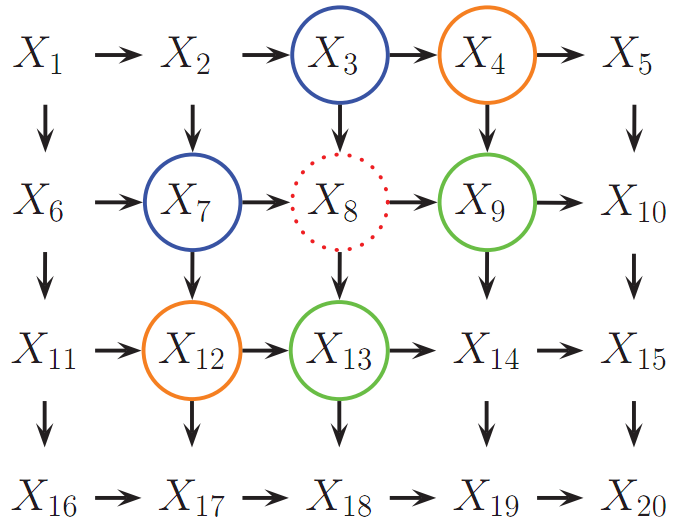
\includegraphics[width=0.5\textwidth]{lattice.png}
\caption{二维晶格状模型}\label{fig:lattice}
\end{figure}

在我们的问题中,由于需要对图像建模,我们采用了如图\ref{fig:lattice}所示的二维晶格状模型,将每个像素点作为模型中的一个未知量(节点),同时相邻像素节点之间存在一条边(edge),表明相邻像素点之间的条件独立关系。

\subsection{我们的模型}
在我们的模型中,给定一幅图像$I$,我们使用一个二值掩图(mask)$Y=\{y_p|p\in I\}$标记出显著物体。图模型以每个像素点为顶点,8领域之间的像素点之间相连,形成一个二维晶格状的概率图。那么,在这个概率图下,$Y$在给定图像$I$下的条件概率可以写为,
\begin{equation}
P(Y|I) = \frac{1}{Z}exp(\sum_{p\in I}F_d(y_p, I) + \sum_{p\in I}\sum_{q\in N_p}F_s(y_p,y_q,I) )
\end{equation}
其中$p$代表$I$中的一个像素点,$y_p$是其显著与否的标记。$F_d(y_p, I)$是“节点特征函数”,$F_s(y_p,y_q,I)$是“邻接边特征函数”,描述了相邻像素点之间的联系。

节点特征函数仅仅与输入的已有显著图$S_i$有关,即
\begin{equation}
F_d(y_p, I) = \sum_{i=1}^{m} \lambda_iS_i(p) + \lambda_{m+1}y_p
\end{equation}
其中$\lambda_i$是条件随机场的一组待学习的参数。而邻接边特征函数描述了相邻像素之间的关系:
\begin{equation}
F_s(y_p,y_q,I) = F_e(y_p,y_q,I) + F_c(y_p,y_q,I)
\end{equation}
其中$F_e(y_p,y_q,I)$考虑到了这样一个事实,如果两个像素点在同一幅显著图中的显著值差别很大,那么他们最后倾向于拥有不同的显著性标记。
\begin{equation}
  F_e(y_p,y_q,I) = \sum_{i=1}^{m}\alpha_i(\textbf{1}(y_p=1,y_q=0)-\textbf{1}(y_p=0,y_q=1))(S_i(p)-S_i(q))
\end{equation}
其中$\alpha_i$为CRF的待学习参数,$\textbf{1}(.)$为指示函数(括号内真为1,假为0)。$F_s$的第二项可以看做一个惩罚项,当像素点的颜色相似却被标上不同的标记时要进行惩罚:
\begin{equation}
F_c(y_p,y_q,I)=\textbf{1}(y_p \not= y_q) exp(-\beta \parallel I(p)-I(q) \parallel )
\end{equation}
其中$\parallel I(p)-I(q) \parallel$代表像素$p$和$q$的颜色差(Lab颜色空间),$\beta$被设置为$(2<\parallel I(p)-I(q) \parallel>^2)^{-1}$,$<.>$代表计算期望。

最后,通过训练这个模型,得到所有参数的最优值。当计算新的显著图时,我们取每个顶点(像素点)被标记为1的概率作为该像素点的显著值。CRF的训练和inference,我们采用了Mark Schmidt的开源工具包UGM\cite{UGM_software}实现。

\section{实验结果}
\subsection{实验方法}
为了评估我们模型的性能,我们采用了Achanta等人创建的公开数据集ASD\cite{achanta2009frequency}。这个数据集包含1000幅图片,每一幅图像都对应有一个人工标注的显著图(二值图,用于标示显著区域)作为Ground Truth。在这个数据集上,我们评估了10种国际上的经典方法作为比较,包括IT\cite{itti1998model}, HC\cite{cheng2011global}, RC\cite{cheng2011global}, SR\cite{hou2007saliency}, AC\cite{achanta2008salient}, FT\cite{achanta2009frequency}, GB\cite{harel2006graph}, IG\cite{achanta2009frequency}, MZ\cite{ma2003contrast} and LC\cite{zhai2006visual}。对于AC,GB,IG,IT,MZ,SR,我直接使用从\cite{achanta2009frequency}上随标准数据集下载的显著图,对于其他方法,我们使用作者提供的公开实现代码。

\subsection{评价标准}
显著区域检测的真正用途在于其应用。我们采用\cite{achanta2009frequency}中的思路,将显著图用于目标物体分割来进行评价。我们首先将显著图采用某个阈值进行二值化,则值为1的像素点为前景物体,值为0的点为背景物体。

试验中,我们采用了固定阈值来二值化显著图,为了评价显著图的质量,阈值从0到255变化,然后分别计算对应的准确率和召回率,最后绘制成准确率-召回率曲线(PR-curve)。

另外,为了进一步评价算法的性能,我们也采用了F-score的评价方式,F-score定义如下:
\begin{equation}
F_{\beta} = \frac{(1+\beta^2)*precision*recall}{\beta^2*precision+recall}
\end{equation}
$\beta^2$用于我们调整对准确率和召回率的重视程度,在我们的试验中被设置为0.3。

\subsection{实验结果}
\begin{figure}
\centering
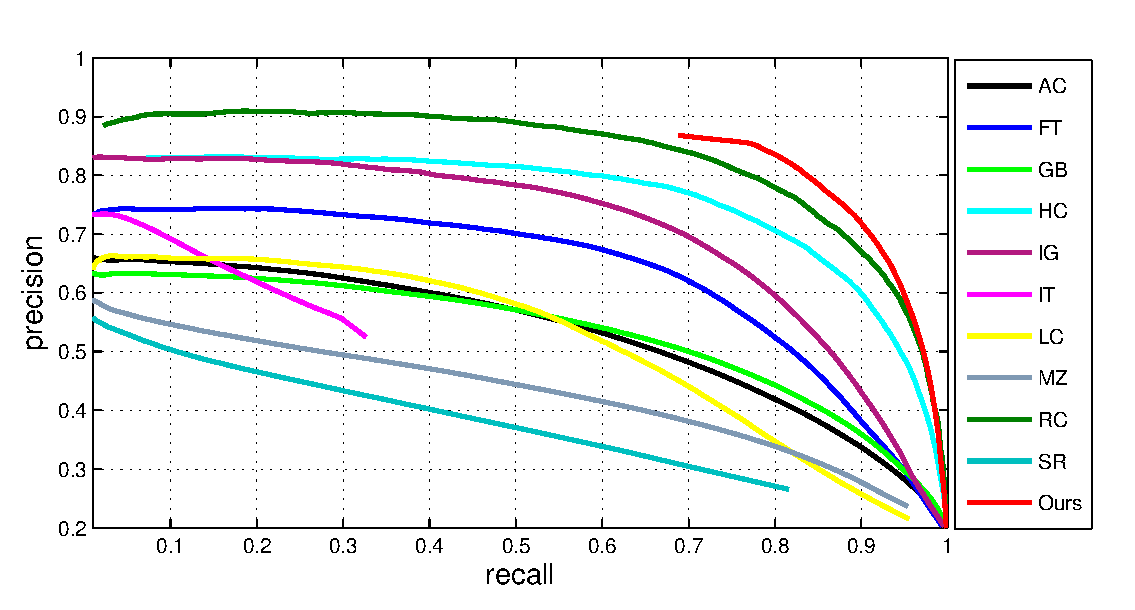
\includegraphics[width=\linewidth]{mrf_pr_curve.eps}
\caption{与其他10种方法的对比:准确率-召回率曲线}
\label{fig:results1_pr}
\end{figure}
PR曲线如图\ref{fig:results1_pr}所示,值得注意的是,我们的方法在任何阈值下都可以达到很高的召回率(>0.7),因此我们的方法是没有召回率低于0.7这部分的曲线的。如果仅仅看召回率大于0.7的部分,我们的方法很显然优于其它方法,拥有更高的准确率。

\begin{figure}
\centering
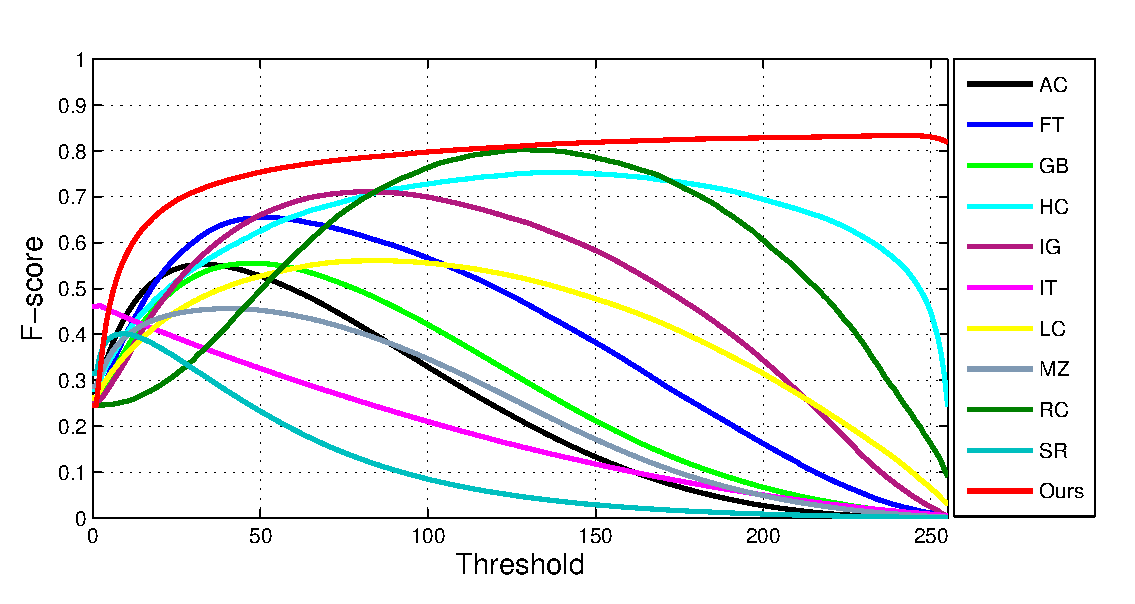
\includegraphics[width=\linewidth]{mrf_f.eps}
\caption{与其他10种方法的对比:F-score曲线}
\label{fig:results1_fscore}
\end{figure}
我们将F-score在各个阈值下的结果绘制成曲线,如图\ref{fig:results1_fscore}所示。看以看到,我们的方法在各个阈值下基本都保持最高的F-score,值得注意的是,我们的方法的F-score在很大的阈值范围内基本保持不变,这说明了我们的方法对阈值不敏感,具有一定的鲁棒性。

我们还提供了一些图片结果的主观对比,如图\ref{fig:vresult1}所示。
\begin{figure}[h]
\centering
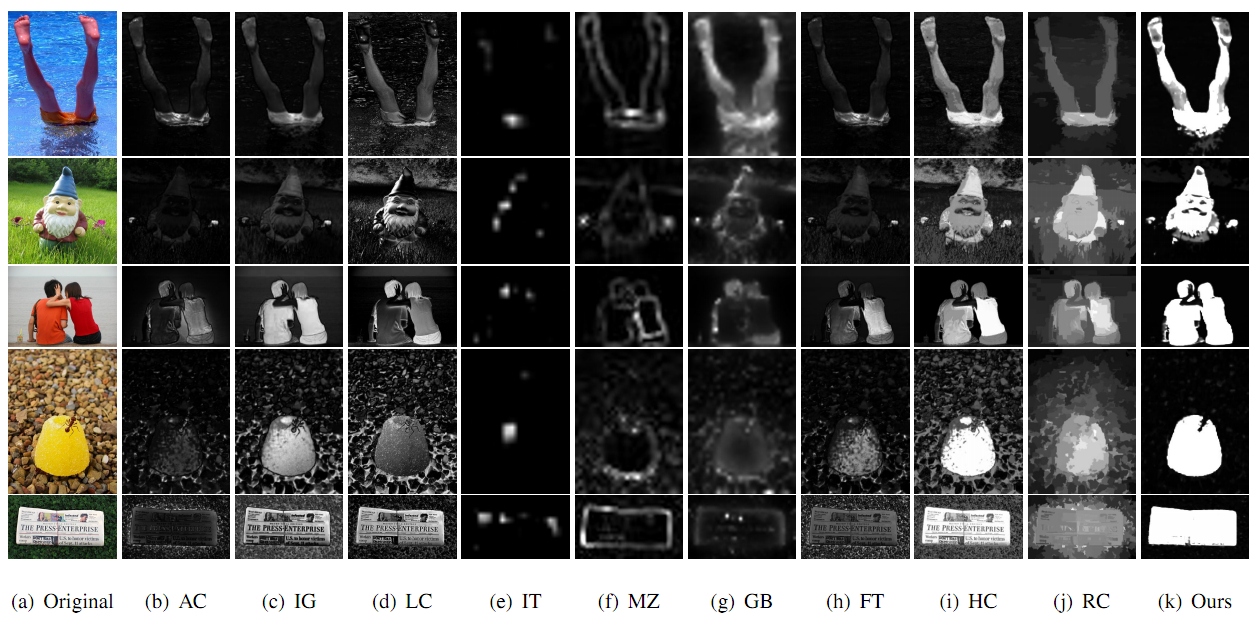
\includegraphics[width=\linewidth]{mrf_vcomp.jpg}
\caption{与其他10种方法的主观视觉对比}\label{fig:vresult1}
\end{figure}